\section{Experiments \& Takeaways}

Before dissecting the internals of LLAP, we take a brief digression into deployments and experiments, 
which add colour to the architectural discussions. 

\subsection{Yahoo Display Network Benchmark}

Yahoo Japan published a timeseries reporting business case as part of a benchmark\cite{impala_perf} comparing
latencies of Cloudera Impala\cite{impala} against Apache Hive. This use-case was based on a production scenario
which features a 500 billion row warehouse which has significant skews in its data distribution. The challenge 
described in the use-case stemmed from having both throughput and latency SLAs and simulated concurrent users
creating extracted reports for further analysis.

The use-case divided produced aggregate of metrics bounded by segments, of selected attributes. The segments 
were primarily the start of the period and the length of the period - daily, weekly, monthly and yearly. The 
attributes were selection criteria which included user demographics and object identifiers. This does not 
easily map into a pre-aggregate MOLAP system as the total number of object identifiers were very large and 
the join against total dimensions produced very little reduction in data, when maintained on a daily basis for
a year.

The query pattern for the time-series had a skew towards the last day and last week, which affects a MPP share-nothing
model adversely by producing a CPU hot-spot around the machines holding the last billion rows. Eventhough Tez was not
affected by that specific issue due to locality delay scheduling, it was still producing secondary network hotspots
around the storage nodes which contained more popular user-demographics. 

This experiment gave valuable feedback into the design of LLAP. Along with use of Tez sessions, the benchmark 
reached an acceptable 5.67 queries per second (20412 queries per hour, exceeding the 15000 queries per hour SLA).

As part of validating LLAP's solution, the exact same benchmark was setup with the latest Hive and run through for the following
query patterns with 20 users, each user getting a unique tuple of parameters.

\begin{itemize}
\item \textbf{Query1x}: aggregate by object id
\item \textbf{Query2x}: aggregate by day
\item \textbf{Query6x}: across 50 object ids by device
\item \textbf{Query7x}: across 50 object ids by day
\end{itemize}

The experimental 50 node cluster had machines with 10Gigabit Ethernet, 20 cores, 128Gb of RAM and 12 disks in each. The LLAP instances
were configured to utilize 96Gb per node, running 24 threads in total with a 10Gb cache. For the purpose of the benchmark, all logging
in LLAP was turned to WARN level to reduce IO overheads. All queries were executed from a single gateway node, over JDBC connections 
and latencies measured are seconds for JDBC submission till last row.

\iffalse
\begin{table}[h]
\begin{tabular}{l|*{4}c}
Query1x  &   Tez (avg)  &   Tez (worst)  &   LLAP (avg)  &   LLAP (worst) \\
\hline
One Day  &   2.53  &   4.5  &   1.33  &   3 \\
One Week  &   3  &   6.18  &   1.37  &   2.9 \\
One Month  &   4  &   7.28  &   1.35  &   2.7 \\
One year  &   7.4  &   19.51  &   3  &   17.22 \\
\end{tabular}
\caption{Query1x across different periods (s)}
\end{table}

\begin{table}[h]
\begin{tabular}{l|*{4}c}
Query2x  &   Tez (avg)  &   Tez (worst)  &   LLAP (avg)  &   LLAP (worst) \\
\hline \\
One Day  &   2.556  &   6.67  &   1.11  &   1.74 \\
One Week  &   1.99  &   2.84  &   1.01  &   1.47 \\
One Month  &   3.07  &   6.65  &   1.29  &   2.2 \\
One year  &   5.03  &   7.47  &   1.74  &   4.67 \\
\end{tabular}
\caption{Query2x across different periods (s)}
\end{table}

\begin{table}[h]
\begin{tabular}{l|*{4}c}
Query6x  &   Tez (avg)  &   Tez (worst)  &   LLAP (avg)  &   LLAP (worst) \\
\hline \\
One Day  &   1.9  &   2.6  &   1.17  &   3.63 \\
One Week  &   2.22  &   5.9  &   1.03  &   1.66 \\
One Month  &   3.5  &   6.7  &   1.23  &   2.76 \\
One year  &   6  &   7.27  &   2  &   5.44 \\
\end{tabular}
\caption{Query6x across different periods (s)}
\end{table}

\begin{table}[h]
\begin{tabular}{l|*{4}c}
Query7x  &   Tez (avg)  &   Tez (worst)  &   LLAP (avg)  &   LLAP (worst) \\
\hline \\
One Day  &   1.9  &   2.6  &   1.17  &   3.63 \\
One Week  &   2.22  &   5.9  &   1.03  &   1.66 \\
One Month  &   3.5  &   6.7  &   1.23  &   2.76 \\
One year  &   6  &   7.27  &   2  &   5.44 \\
\end{tabular}
\caption{Query7x across different periods (s)}
\end{table}
\fi

\begin{figure}[bthp]
\centering
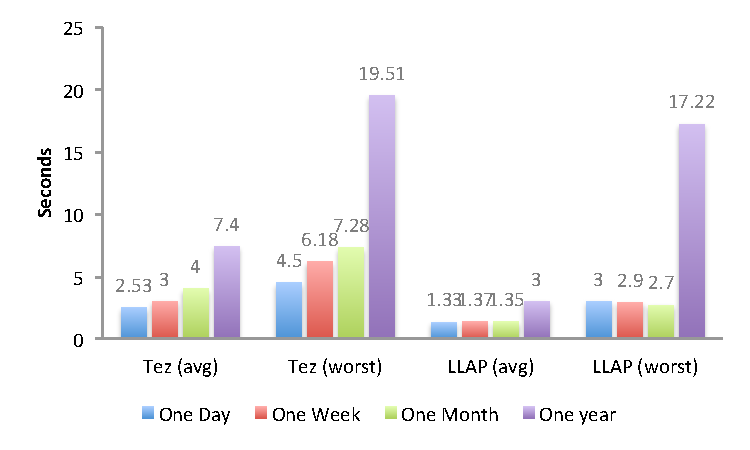
\includegraphics[width=0.9\columnwidth]{figures/q1x.pdf}
\caption{Query1x across different periods (s)}
\label{fig:q1x}
\end{figure} 

\begin{figure}[bthp]
\centering
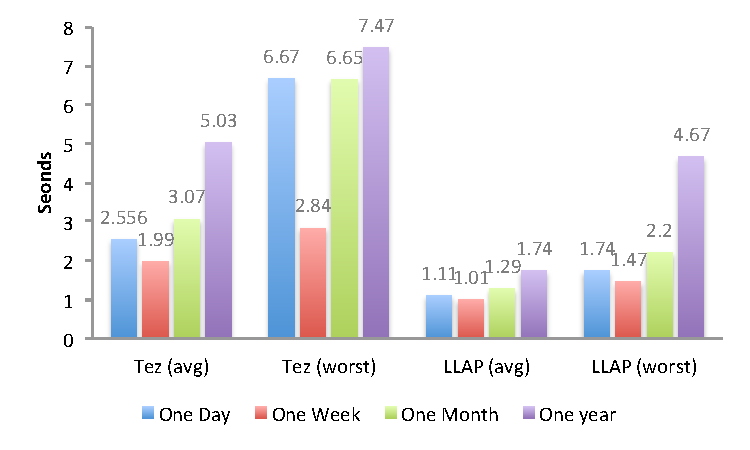
\includegraphics[width=0.9\columnwidth]{figures/q2x.pdf}
\caption{Query2x across different periods (s)}
\label{fig:q2x}
\end{figure} 

\begin{figure}[bthp]
\centering
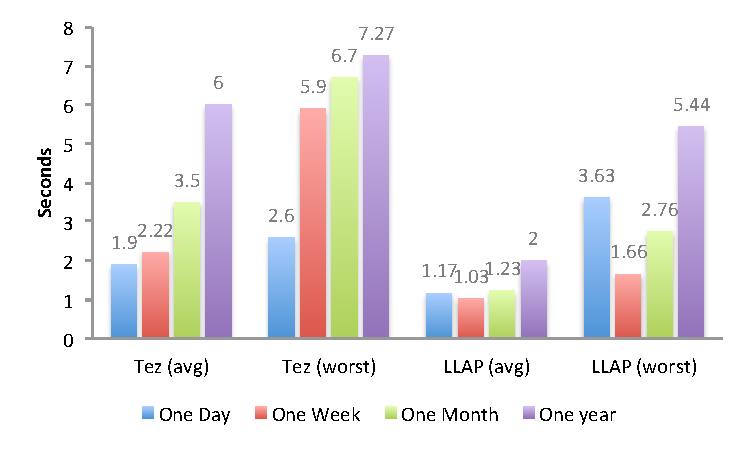
\includegraphics[width=0.9\columnwidth]{figures/q6x.pdf}
\caption{Query6x across different periods (s)}
\label{fig:q6x}
\end{figure} 

\begin{figure}[bthp]
\centering
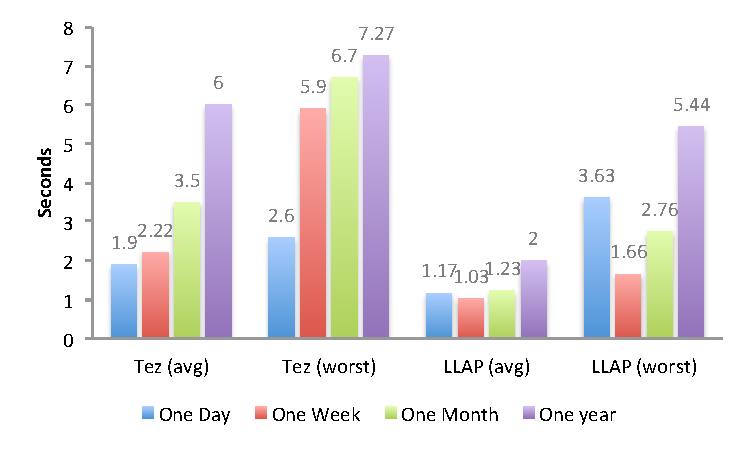
\includegraphics[width=0.9\columnwidth]{figures/q7x.pdf}
\caption{Query7x across different periods (s)}
\label{fig:q7x}
\end{figure} 


LLAP managed to lower the latency as well as hit a far higher throughput of 15.16 q/s (54576 queries per hour). The 
performance bottlenecks with LLAP had moved from the data skew towards the cpu utilized by the bottlenecks within
the JDBC layer in HiveServer2. This was isolated from the use-case by increasing the total number of users in the system and
increasing the number of HiveServer2 until worst case latencies dropped out of SLA.


\begin{figure}[!h]
\centering
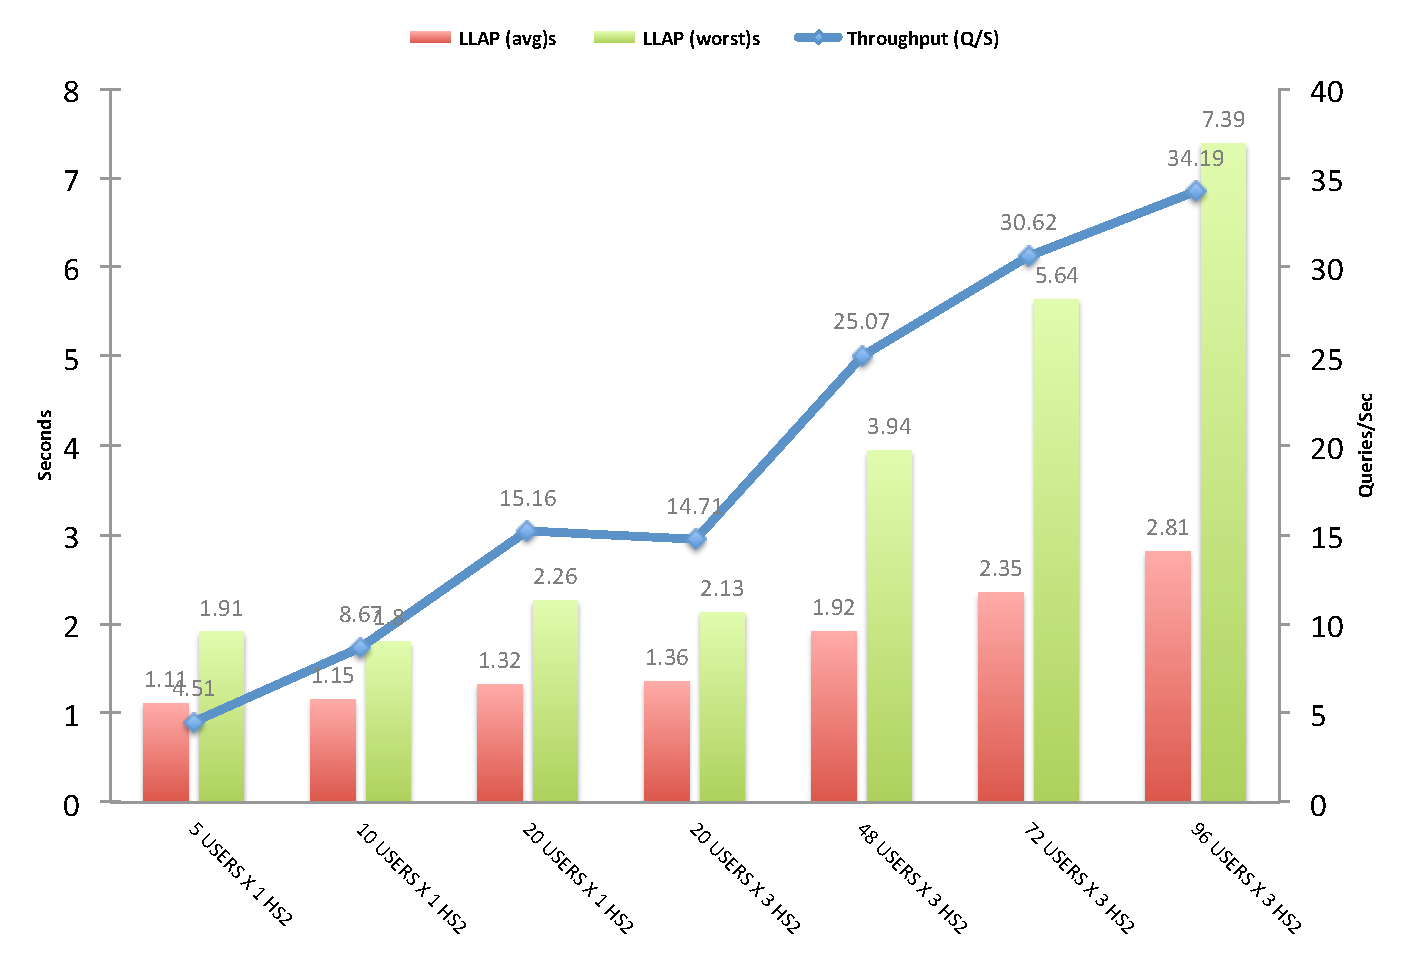
\includegraphics[width=0.9\columnwidth]{figures/throughput.pdf}
\label{fig:throughput}
\caption{HiveServer2 Concurrency Tests}
\end{figure}

\iffalse
\begin{table}[H]
\begin{tabular}{l|*{3}c}
Concurrency & Throughput (Q/S) & LLAP(avg)s & LLAP (worst)s \\
\hline \\
5 Users x 1 HS2 & 4.51 & 1.11 & 1.91 \\
10 Users x 1 HS2 & 8.67 & 1.15 & 1.8 \\
20 Users x 1 HS2 & 15.16 & 1.32 & 2.26 \\
20 Users x 3 HS2 & 14.71 & 1.36 & 2.13 \\
48 Users x 3 HS2 & 25.07 & 1.92 & 3.94 \\
72 Users x 3 HS2 & 30.62 & 2.35 & 5.64 \\
96 Users x 3 HS2 & 34.19 & 2.81 & 7.39 \\
\end{tabular}
\caption{HiveServer2 Concurrency Tests}
\end{table}
\fi

\subsection{TPC-DS Interactive Queries}

\begin{figure}[bthp]
\centering
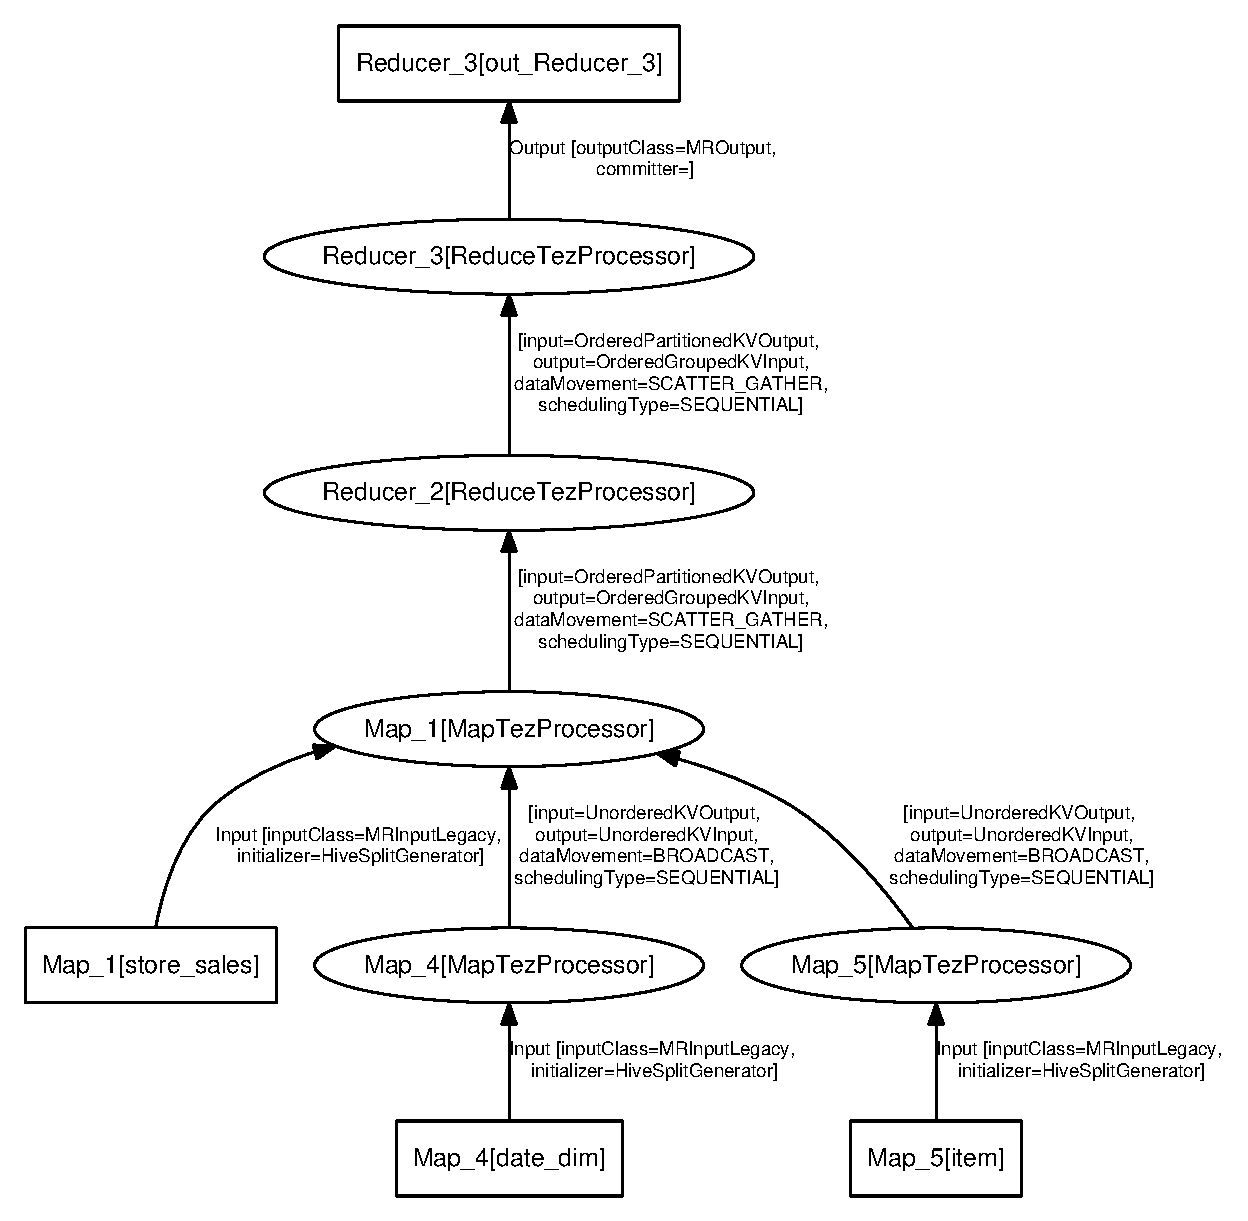
\includegraphics[width=0.8\columnwidth]{figures/q55.eps}
\caption{Query55: DAG Plan}
\label{fig:q55}
\end{figure} 

The TPC-DS data-set is a better candiate for a repeatable benchmark for LLAP, allowing any cluster to generate
identical data at scale factors for testing. The experimental setup is a \emph{SCALE=1000} TPC-DS data set generated
and loaded using the schema from hive-testbench\cite{testbench}, with interactive set of 27, 42, 52, 55, 68, 73 and 98, 
without introducing any partition filters on the queries.

These are all multi-stage queries from a MapReduce context, with internal shuffle distribution edges. For example, 
Query 55 DAG plan is illustrated in figure~\ref{fig:q55}.  

Benchmarked on a Hadoop 2.7.1 cluster, with following hardware configuration.

\begin{itemize}
\item 2x Intel(R) Xeon(R) CPU E5-2640 v2 @ 2.00GHz for total of 16 CPU cores/machine
\item 256GB RAM per node
\item 6x 4TB WDC WD4000FYYZ-0 drives per node
\item 10 Gigabit interconnect between the nodes
\end{itemize}

The LLAP instances were created with 128Gb of working set memory, 32Gb of cache and 16 executor threads per
instance. The following configurations were applied to the Hive planner to produce consistent cache coherent 
runs during benchmarking.

\begin{itemize}
\item hive.llap.task.scheduler.locality.delay=-1;
\item hive.llap.client.consistent.splits=true;
\item hive.optimize.reducededuplication.min.reducer=1;
\end{itemize}

\iffalse
\begin{table}[h]
\begin{tabular}{l|*{1}cr}
Query & LLAP time(s)\\
\hline \\
Query 27 & 3.13  \\
Query 42 & 0.98  \\
Query 52 & 1.05  \\
Query 55 & 1.76  \\
Query 68 & 4.77  \\
Query 73 & 1.90  \\
Query 98 & 5.36  \\
\end{tabular}
\caption{Interactive Queries on LLAP}
\end{table}
\fi

\begin{figure}[bthp]
\centering
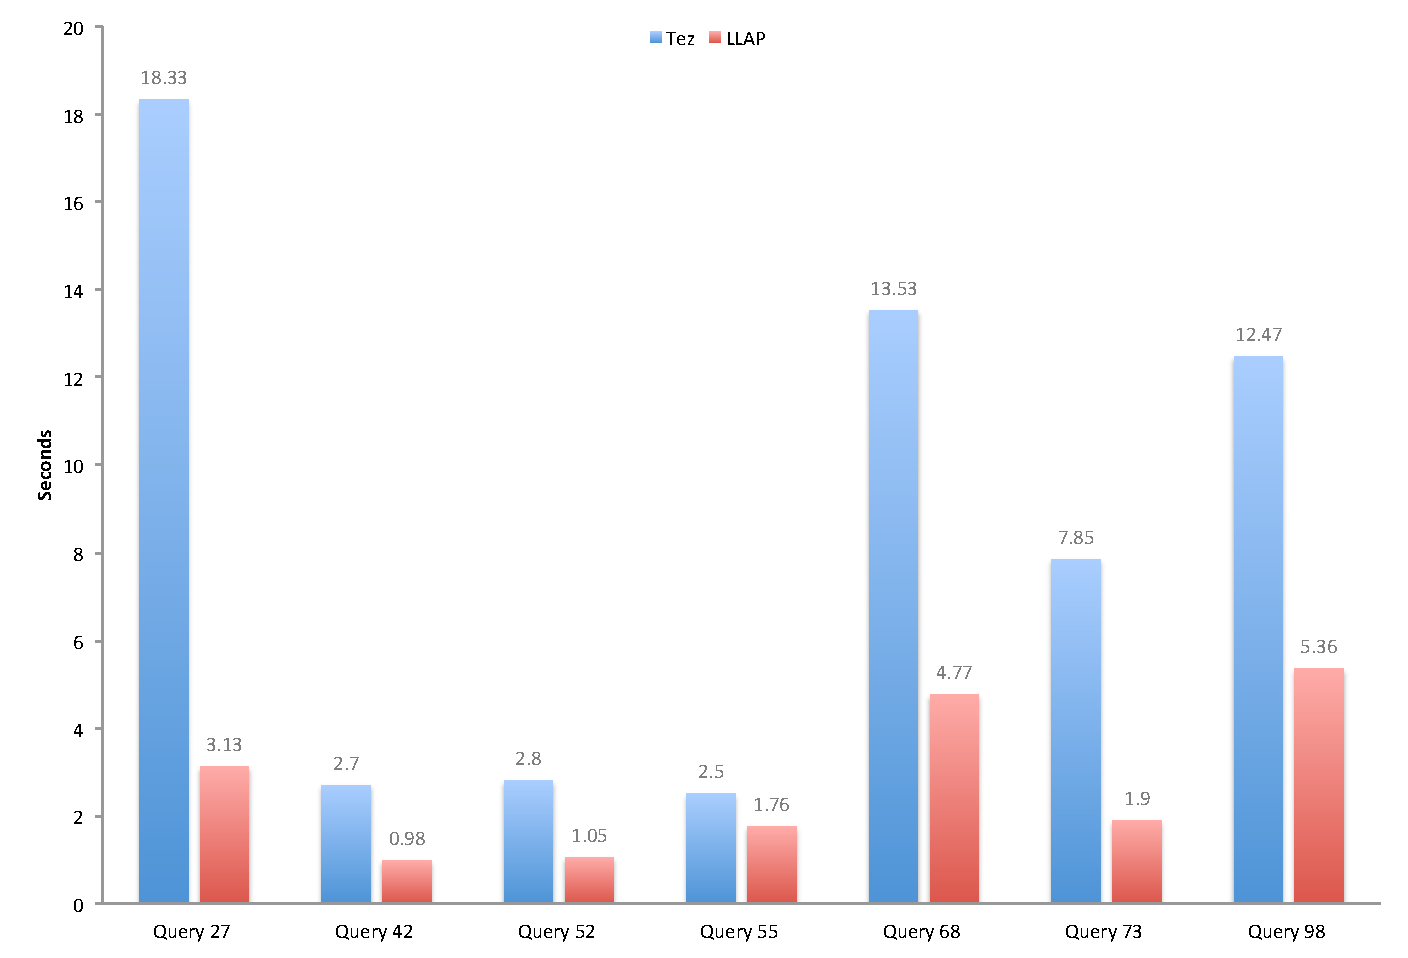
\includegraphics[width=0.8\columnwidth]{figures/tpc-ds.pdf}
\caption{Interactive queries: LLAP vs Tez}
\label{fig:llap_v_tez}
\end{figure} 

The queries 42, 52 \& 55, can run at the similar latencies even when using a single LLAP instance to compare against, since they process
approximately 93 million rows, which is less than the single node processing rate of LLAP clocked at approximately 115 million rows per second  
for ORC.
